\subsection{Valutazione dell'usabilità}

    \begin{flushleft}
       Per la valutazione dell'usabilità del nostro applicativo a priori, cioè prima della fase di sviluppo vera a propria,
       abbiamo deciso di imporci come linee guida le euristiche di Nielsen.
       Ne sono 10, ma vorremmo richiamare l'attenzione su alcune di esse nello specifico:
        \begin{itemize}
            \item  \emph{Visibilità dello stato del sistema.} Il sistema presentava una discreta mancanza di feedback, che prevediamo di colmare con elementi quali Dialog, Toast, AlertDialog e SnackBar.
            \item  \emph{Prevenzione degli errori.} Il sistema reagisce in maniera controllata e predeterminata alle situazioni di errori che gli utenti possono causare. Nulla è lasciato al caso, ed è, nelle build provate dal team, gestita qualsiasi azione eseguibile dagli utenti.
            \item  \emph{Riconoscere piuttosto che ricordare.} La nostra app è dotata di sezioni ben distinte, interfacce dinamiche a seconda del tipo di utente che le usa, e icone e testi ecplicativi dell'azione che si va a intrapendere.
            \item  \emph{Guida e documentazione.} E' presente un simpatico topolino (che richiama il logo dell'app) che consiglia tramite vignette e piccoli dialoghi le azioni che si possono intraprendere. Inoltre ci sono piccole note come campi obbligatori ecc.
        \end{itemize}
    \end{flushleft}

    \begin{figure}[H]
        \centering
        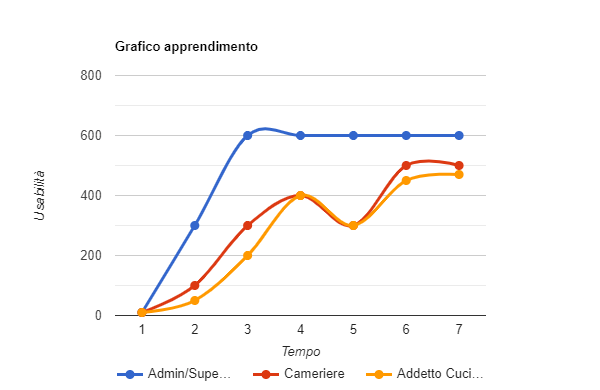
\includegraphics[scale=0.6]{assets/diagrammi/immagini varie/grafico usabilita.png}
        \caption{\textbf{Grafico}: Usabilità}\label{fig:Usabilità_graph}
    \end{figure}